\documentclass[12pt]{report}
\usepackage[T1]{fontenc}
\usepackage[utf8]{inputenc} 
\usepackage[margin=1in]{geometry}
\usepackage{graphicx}
\usepackage{float}
\usepackage{datetime}
\newcommand{\Logo}{
    \begin{figure}[H]
        \centering
        
\includegraphics[height=0.3\textwidth]{../Resources/politechnika_sl_logo_bw_pion_pl.pdf}
    \end{figure}
}

\usepackage{hyperref}
\hypersetup{
    colorlinks=true,
    urlcolor=black,
    linkcolor=black
}


\begin{document}

\begin{titlepage}
    \Logo
    \centering
    \vspace*{1in}

    % --- Title Section ---
    \huge
    \textbf{Starbucks Customer Ordering Patterns} \\
    \vspace{0.5in}

    \large
    \textbf{Analysis of the ``Digital Venti Effect''} \\
    \vspace{1.5in}

    % --- Author Section ---
    \textbf{Prepared by:} \\
    \vspace{0.2in}
    Zuzanna Safaryjska \\
    Mateusz Pyrek \\
    Adam Dyrda \\
    Oliwier Jędrzejczyk \\
    \vfill


    Academic Year 2025/2026 \\
    %to do: add date, add polsl logo

    % --- Footer Section ---

\end{titlepage}

\tableofcontents
\newpage

\chapter{General description of the dataset}
\noindent The subject of the project is a statistical analysis of the ``Starbucks Customer Ordering Patterns'' dataset. This dataset, which was published on Kaggle, consists of 100 000 real transactions made by Starbucks customers over a two-year period (2024-2025). It allows to analyse customer behavior, focusing on how orders are placed, the financial value of those orders, and the time required for fulfillment. To ensure the methods are adjusted to the dataset, five key features have been isolated to analyze trends in spending, demographic preferences, and operational efficiency.

\section{Attributes of the dataset}
Below there is a list of all attributes of the dataset.
\begin{itemize}
    \item IDs:
          \begin{itemize}
              \item customer \_id: unique identifier for each customer (15000 unique profiles),
              \item order\_id: unique transaction id (100 000 orders),
              \item store\_id: identifier for each store,
          \end{itemize}
\end{itemize}
\begin{itemize}
    \item Date:
          \begin{itemize}
              \item order\_date: (ranging from 01.2024 to 12.2025),
              \item order\_time,
              \item day\_of\_week,
          \end{itemize}
\end{itemize}
\begin{itemize}
    \item Order:
          \begin{itemize}
              \item order\_channel: method used to place the order (Mobile App, Drive-Thru, In-Store Cashier or Kiosk),
              \item store\_location\_type: (Urban, Suburban or Rural)
              \item region: (Northeast, Southeast, Midwest, West or Southwest),
              \item customer\_age\_group: (18-24, 25-34, 35-44, 45-54 or 55+),
              \item customer\_gender: (Male, Female or Other),
              \item is\_rewards\_member: whether the customer is a member of the Starbucks Rewards program (True or False),
              \item cart\_size: number of items in the order,
              \item num\_customizations: number of modifications made to the order (extra shots, syrup, different milk),
              \item total\_spend: total cost of the transaction in USD\@,
              \item fulfillment\_time\_min: time (in minutes) from the moment the order is placed until it is ready for the customer,
              \item drink\_category: (Coffee, Tea, Refresher or Other),
              \item has\_food\_item: (True or False),
              \item order\_ahead: whether the order was placed ahead of time (True or False),
              \item customer\_satifsaction: rating from 1 to 5 (correlated with fulfillment time and channel),

          \end{itemize}
\end{itemize}

\pagebreak

\section{Summary of selected attributes}

%add some information about the dataset; the origin, how many elememts are in the set, short description of all attributes, some of them described, 

%Order Channel

\subsection{order\_channel}
\subsubsection{description}
This feature lists which method of ordering was used by the customer while
placing order. Available options were Mobile App, Drive-Thru, In-Store Cashier,
Kiosk.
\subsubsection{graph representation}
%import of the pie chart

In figure \ref{fig:order_channel_pie} we can see graphical representation of order channels
\begin{figure}[H]

    \centering
    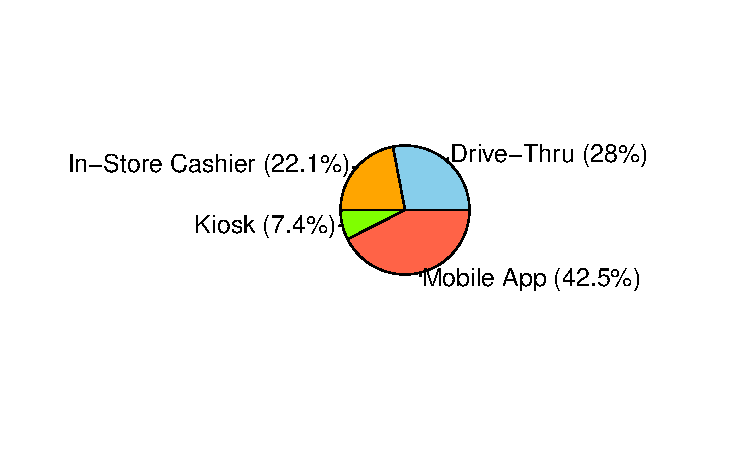
\includegraphics[width=0.8\textwidth]{../Resources/Charts/order_channel_pie_chart.pdf}
    \caption{Percentage distribution of order channels}
    \label{fig:order_channel_pie}
\end{figure}

\subsubsection{use-case}
We will use this feature to check how customers were placing orders.


%total spent
\subsection{total\_spend}
\subsubsection{description}
\noindent This feature shows the total cost of the transaction in USD\@.
\subsubsection{graph representation}
%import of the histogram
\begin{figure}[H]

    \centering
    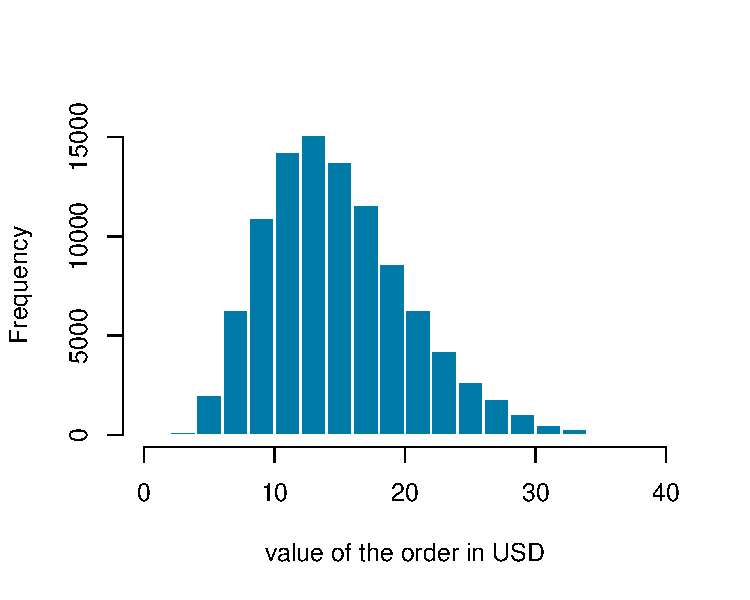
\includegraphics[width=0.8\textwidth]{../Resources/Charts/total_spend_histogram.pdf}
    \caption{Distribution of total spend among customers}
    \label{fig:total_spend_histogram}
\end{figure}

\subsubsection{use-case}
\noindent We will use this data and compare it to the order\_channel to check if there exists a relation between the method of ordering and the amount spent.

%num customizations - Zuzia robi
\subsection{num\_customizations}
\subsubsection{description}
\noindent This feature shows the number of modifications made to the order (e.g., extra shots, syrup, milk sub).
\subsubsection{graph representation}
%import of the ...
\begin{figure}[H]

    \centering
    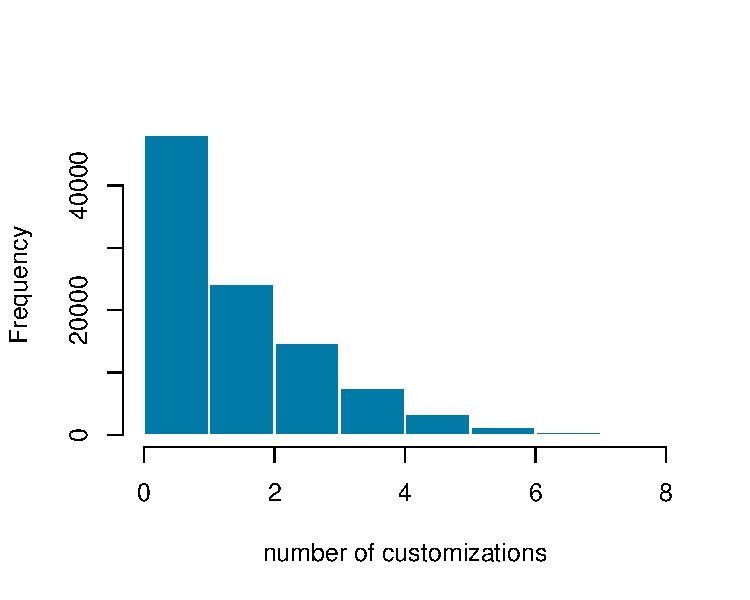
\includegraphics[width=0.8\textwidth]{../Resources/Charts/num_customizations_histogram.pdf}
    \caption{Distribution of the number of customizations among customers}
    \label{fig:num_customizations_histogram}
\end{figure}
\subsubsection{use-case}
\noindent We will use this data to check if mobile app users demonstrate higher tendency to customizing their orders.

%customer age group - Mateusz robi
\subsection{customer\_age\_group}
\subsubsection{description}
\noindent This feature shows the age group of the customer.
\subsubsection{graph representation}
%import of the bar chart
\begin{figure}[H]

    \centering
    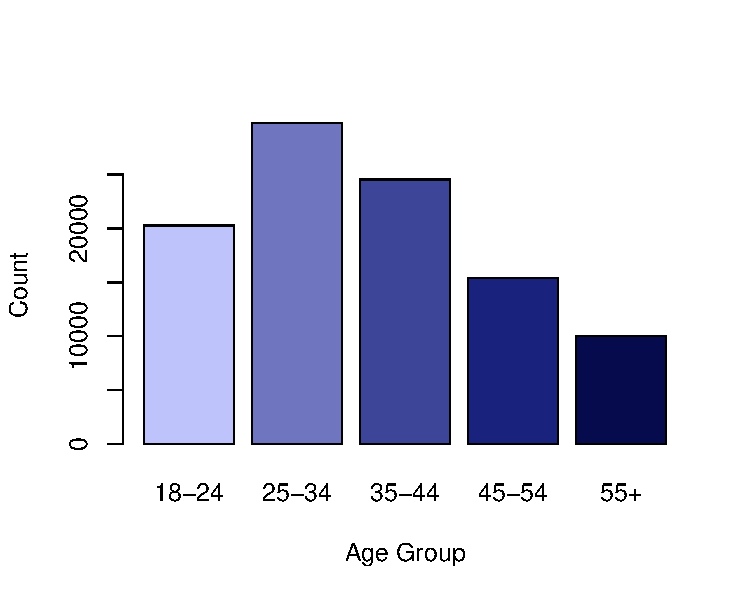
\includegraphics[width=0.8\textwidth]{../Resources/Charts/customer_age_group_bar_chart.pdf}
    \caption{Distribution of customer age groups}
    \label{fig:customer_age_group_bar}
\end{figure}

\subsubsection{use-case}
\noindent A relationship between customer age groups and their ordering behavior will be investigated, notably whether certain age groups prefer eg. specific order channels or spend more money.


%fulfillment time - Oliwier robi
\subsection{fulfillment\_time\_min}
\subsubsection{description}
\noindent This feature measures the time (in minutes) from the moment the order is placed until it is ready for the customer. It is a key metric for operational efficiency.
\subsubsection{graph representation}
% import of the bar chart for fulfillment time
\begin{figure}[H]

    \centering
    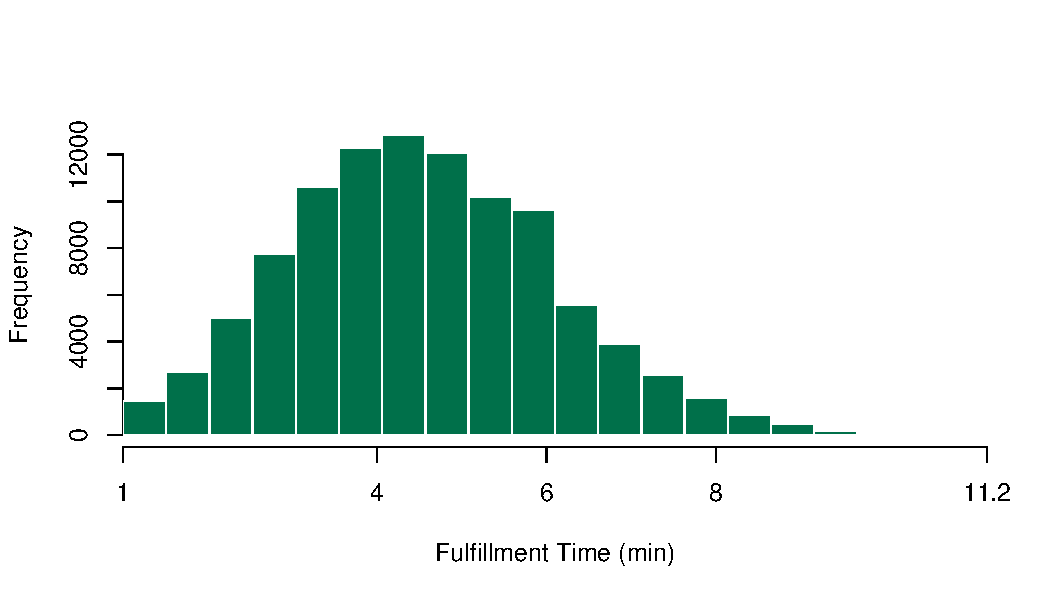
\includegraphics[width=0.8\textwidth]{../Resources/Charts/fulfillment_time_histogram.pdf}
    \caption{Distribution of fulfillment time among customers}
    \label{fig:fulfillment_time_histogram}
\end{figure}

\subsubsection{use-case}
\noindent We will analyze this attribute to determine how the complexity of an order (number of customizations) affects service speed. This helps identify whether encouraging modifications leads to operational bottlenecks.

\chapter{Calculation of descriptive statistics}
\section{Descriptive statistics by attribute}
\subsection{order\_channel}
\noindent As the order\_channel is presented as a string, we will calculate the mode and cardinality to understand the distribution of ordering methods among customers. This will help us identify which channels are most popular and if there are any significant differences in customer preferences.

\begin{table}[H]

    \centering
    \begin{tabular}{|l|l|l|}
        \hline
        Measure of a central tendency & Obtained result \\ \hline
        mode                          & 25-34           \\ \hline
        cardinality                   & 5               \\ \hline
    \end{tabular}
    \caption{Descriptive statistics for order\_channel}
    \label{tab:desc_order_channel}
\end{table}

\subsection{total\_spend}
\noindent As the total\_spend is a continuous numerical variable, we will calculate the mean, median, mode, standard deviation, range, 0.25 quartile, and 0.75 quartile to understand the distribution of spending amounts among customers. This will help us identify average spending patterns, variability in transaction values, and whether there are significant outliers in customer expenditures.

\begin{table}[H]

    \centering
    \begin{tabular}{|l|l|l|}
        \hline
        Measure of a central tendency & Obtained result  \\ \hline
        mean value                    & 14.8667708       \\ \hline
        median value                  & 14.17            \\ \hline
        mode value                    & 12.1453342509566 \\ \hline
        range                         & 3.51 - 40.31     \\ \hline
        standard deviation            & 5.50680009558536 \\ \hline
        0.25 Quartile                 & 10.8375          \\ \hline
        0.75 Quartile                 & 18.18            \\ \hline
    \end{tabular}
    \caption{Descriptive statistics for total\_spend}
    \label{tab:desc_total_spend}
\end{table}

\subsection{num\_customizations}
\noindent As num\_customizations is a discrete numerical variable, we will calculate the mean, median, mode, standard deviation, range, 0.25 quartile, and 0.75 quartile to understand the distribution of order modifications among customers. This will help us identify average customization patterns, variability in the number of modifications per order, and whether certain customers tend to customize their orders significantly more than others.

\begin{table}[H]

    \centering
    \begin{tabular}{|l|l|l|}
        \hline
        Measure of a central tendency & Obtained result   \\ \hline
        mean value                    & 1.81077           \\ \hline
        median value                  & 2                 \\ \hline
        mode value                    & 0.998356888479198 \\ \hline
        range                         & 0 - 8             \\ \hline
        standard deviation            & 1.46279985129078  \\ \hline
        0.25 Quartile                 & 1                 \\ \hline
        0.75 Quartile                 & 3                 \\ \hline
    \end{tabular}
    \caption{Descriptive statistics for num\_customizations}
    \label{tab:desc_num_customizations}
\end{table}
\subsection{customer\_age\_group}
\noindent As the customer\_age\_group is presented as a string, we will calculate the mode and cardinality to understand the distribution of age groups among customers. This will help us identify which age groups are most represented and if there are any significant differences in customer preferences.

\begin{table}[H]

    \centering
    \begin{tabular}{|l|l|l|}
        \hline
        Measure of a central tendency & Obtained result \\ \hline
        mode                          & 25-34           \\ \hline
        cardinality                   & 5               \\ \hline
    \end{tabular}

    \caption{Descriptive statistics for customer\_age\_group}
    \label{tab:desc_customer_age_group}
\end{table}
\subsection{fulfillment\_time\_min}
\noindent As the fulfillment\_time\_min is a continuous numerical variable, we will calculate the mean, median, mode, standard deviation, range, 0.25 quartile, and 0.75 quartile to understand the distribution of fulfillment times among customers. This will help us identify average fulfillment patterns, variability in delivery times, and whether there are significant outliers in customer delivery experiences.

\begin{table}[H]

    \centering
    \begin{tabular}{|l|l|l|}
        \hline
        Measure of a central tendency & Obtained result  \\ \hline
        mean value                    & 4.54608          \\ \hline
        median value                  & 4.4              \\ \hline
        mode value                    & 4.31807337490211 \\ \hline
        range                         & 1 - 11.2         \\ \hline
        standard deviation            & 1.55026948204314 \\ \hline
        0.25 Quartile                 & 3.4              \\ \hline
        0.75 Quartile                 & 5.5              \\ \hline
    \end{tabular}
    \caption{Descriptive statistics for fulfillment\_time\_min}
    \label{tab:desc_fulfillment_time}
\end{table}
\chapter{Testing of the hypothesis about the normality of distributions}
\section{Formulation of the Hypotheses}
To determine the appropriate statistical methods for further analysis, it is necessary to test whether the continuous variables in the dataset specifically the total cost of the transaction (total\_spend) and the time from order placement to completion (fulfillment\_time\_min) — follow a normal (Gaussian) distribution.
For each of these variables, the following statistical hypotheses are established:
\begin{itemize}
    \item $\mathbf{H_0}$:The distribution of the analyzed variable follows a normal distribution.
    \item $\mathbf{H_1}$:The distribution of the analyzed variable does not follow a normal distribution.

\end{itemize}
The adopted level of significance for all statistical tests in this report is alpha=0.05.
\section{Visual Assessment Using Q-Q Plots}
To initially assess the distribution of the continuous variables, Quantile-Quantile (Q-Q) plots were generated. A Q-Q plot compares the quantiles of the sample data against the theoretical quantiles of a perfectly normal distribution. If the observed data is normally distributed, the data points will align closely with the diagonal reference line.
\subsection{total\_spend}
\begin{figure}[H]
    \centering
    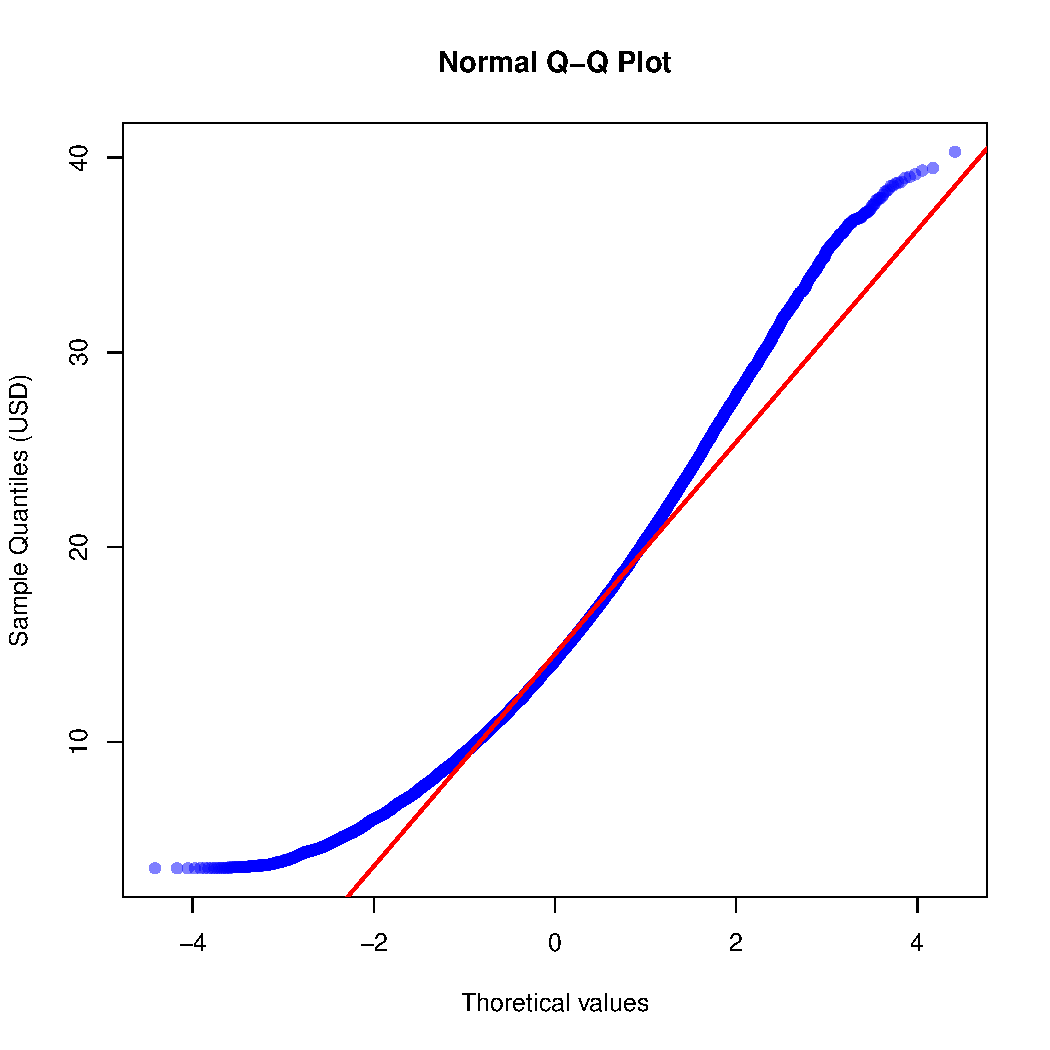
\includegraphics[width=0.8\textwidth]{../Resources/Charts/Normality_testing/total_spend_Q-Q.pdf}
    \caption{Normal Q-Q Plot for total\_spend}
    \label{fig:total_spend_qq}
\end{figure}
As observed in \ref{fig:total_spend_qq}, the data points for the total cost of the transaction (total\_spend)  align closely with the reference line in the central quantiles. However, deviations are visible at the both uper and lower extremes, indicating the presence of outliers at both ends of the spending spectrum.
\subsection{fulfillment\_time\_min}
\begin{figure}[H]
    \centering
    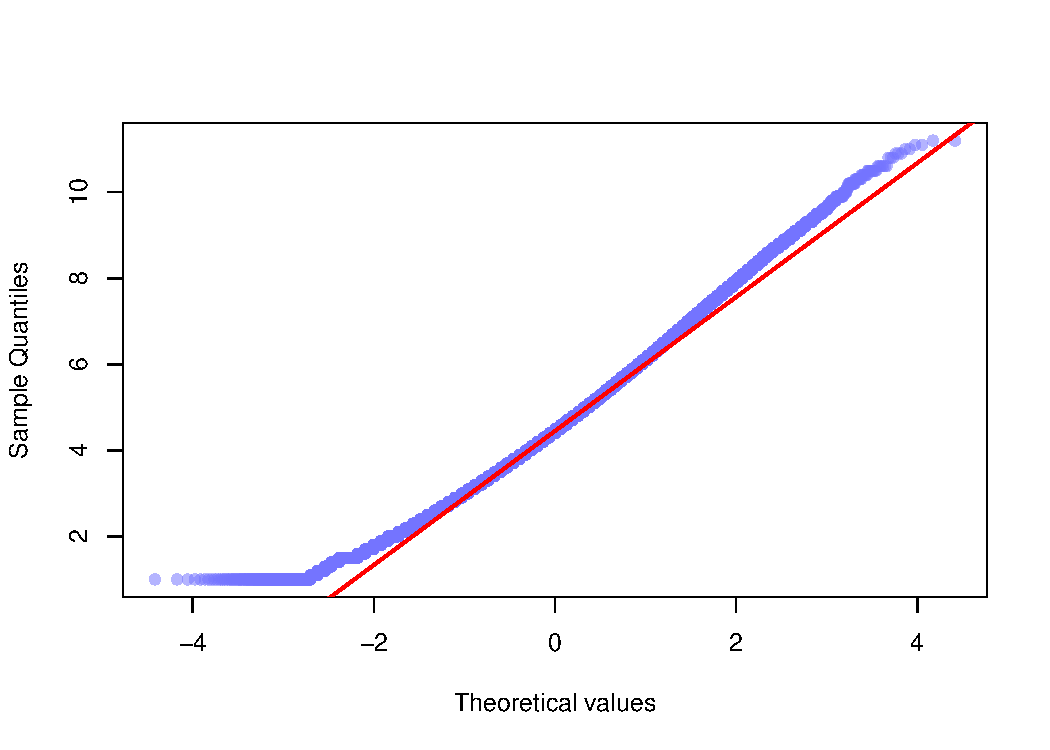
\includegraphics[width=0.8\textwidth]{../Resources/Charts/Normality_testing/fulfillment_Q-Q.pdf}
    \caption{Normal Q-Q Plot for fulfillment\_time\_min}
    \label{fig:fulfillment_time_qq}
\end{figure}
As illustrated in \ref{fig:fulfillment_time_qq}, the Normal Q-Q plot for fulfillment\_time\_min demonstrates strong alignment with the reference line across the central and upper quantiles. However the data exhibits a strict floor effect on the left tail, reflecting the physical minimum time boundary required to fulfill an order.

\section{Analysis of Skewness and Kurtosis}
To quantitatively assess the shape of the data distributions, skewness and kurtosis were calculated. As a statistical baseline, a perfectly symmetrical normal distribution has a skewness of exactly 0 and a kurtosis of 3.0; deviations from these figures indicate directional skew and the presence of extreme outliers, respectively.
\subsection{total\_spend}
\begin{table}[H]

    \centering
    \begin{tabular}{|l|l|l|}
        \hline
        Measure  & Obtained result  \\ \hline
        Skewness & 0.67007900905166 \\ \hline
        Kurtosis & 3.37746288170318 \\ \hline
    \end{tabular}

    \caption{Skewness and Kurtosis results for total\_spend}
    \label{tab:skew_kurt_total_spend}
\end{table}
The total\_spend variable exhibits a moderate positive skewness (0.67) and a kurtosis of 3.38, indicating a right-skewed distribution with slightly heavier tails than a standard normal curve due to a subset of high-value transactions.
\subsection{fulfillment\_time\_min}
\begin{table}[H]

    \centering
    \begin{tabular}{|l|l|l|}
        \hline
        Measure  & Obtained result   \\ \hline
        Skewness & 0.363767571948986 \\ \hline
        Kurtosis & 2.98159553637017  \\ \hline
    \end{tabular}

    \caption{Skewness and Kurtosis results for fulfillment\_time\_min}
    \label{tab:skew_kurt_fulfillment_time}
\end{table}
The fulfillment\_time\_min variable displays near-perfect symmetry with a minimal skewness of 0.36 and a kurtosis of 2.98, demonstrating that its tail behavior aligns almost perfectly with a theoretical normal distribution.
\section{Formal Hypothesis Testing (Kolmogorov-Smirnov)}
To conclusively determine whether the data follows a normal distribution, a Kolmogorov-Smirnov (K-S) test was conducted. The K-S test operates by comparing the actual distribution of the dataset against a theoretically perfect normal curve. In this test, the null hypothesis assumes that the data is perfectly normal. The resulting p-value indicates the probability of seeing the current data if it were truly normal; a p-value below the standard threshold of 0.05 means we must reject the null hypothesis and conclude that the data significantly deviates from a normal distribution.
\subsection{total\_spend}
\begin{table}[H]

    \centering
    \begin{tabular}{|l|l|l|}
        \hline
        Measure              & Obtained result    \\ \hline
        D (maximum distance) & 0.051314           \\ \hline
        p-value              & $2.2\cdot10^{-16}$ \\ \hline
    \end{tabular}

    \caption{Kolmogorov-Smirnov test results for total\_spend}
    \label{tab:ks_total_spend}
\end{table}
For the total\_spend variable, the K-S test returned p-value equal $2.2\cdot10^{-16}$
Because this p-value is vastly smaller than 0.05, we decisively reject the null hypothesis $H_0$, confirming that the distribution of total spend is not normal.
\subsection{fulfillment\_time\_min}
\begin{table}[H]

    \centering
    \begin{tabular}{|l|l|l|}
        \hline
        Measure              & Obtained result    \\ \hline
        D (maximum distance) & 0.039321           \\ \hline
        p-value              & $2.2\cdot10^{-16}$ \\ \hline
    \end{tabular}

    \caption{Kolmogorov-Smirnov test results for fulfillment\_time\_min}
    \label{tab:ks_fulfillment_time}
\end{table}
Similarly the p-value for  fulfillment\_time\_min equals $2.2\cdot10^{-16}$.
Therefore, we also reject the null hypothesis $H_0$, for this metric, concluding that fulfillment time does not follow a perfectly normal distribution.
\section{Conclusion on Normality}
Based on visual, descriptive, and formal mathematical testing, we conclude that the distribution of both total\_spend and fulfillment\_time\_min deviates from strict normality.
For total\_spend, this deviation is driven by a small number of extreme high-value purchases that stretch the data upward. For fulfillment\_time\_min, the data is highly symmetrical but is cleanly truncated by a 1-minute physical minimum required to fulfill an order. Ultimately, these results perfectly reflect the real-world operational realities of the business: transaction values have no ceiling, and fulfillment times have a hard physical floor.
\chapter{Expected relationships between the attributes}
\chapter{Additional analyses aka something new}
\chapter{Results and conclusions}
\end{document}
